\documentclass[compsoc,12pt,a4paper]{IEEEtran}
\usepackage{blindtext}
\usepackage{color}
\usepackage[margin=2cm]{geometry}
\usepackage{graphicx}
\usepackage{listings}
\usepackage{tikz}
\usetikzlibrary{shapes,arrows}
\usepackage{wrapfig}

\definecolor{dkgreen}{rgb}{0,0.6,0}
\definecolor{gray}{rgb}{0.5,0.5,0.5}
\definecolor{mauve}{rgb}{0.58,0,0.82}

\lstset{ 	frame=none,
				aboveskip=3mm,
				belowskip=3mm,
			  	showstringspaces=false,
			 	columns=flexible,
			 	basicstyle={\small\ttfamily},
				numbers=none,
			  	numberstyle=\tiny\color{gray},
			  	keywordstyle=\color{blue},
			  	commentstyle=\color{dkgreen},
			  	stringstyle=\color{mauve},
			  	breaklines=true,
			 	breakatwhitespace=true,   
			  	tabsize=3, 
			  	escapeinside={(**}{*)}	}

\usepackage{cite}
\graphicspath{{./img/}}
\DeclareGraphicsExtensions{.PNG}
\usepackage[cmex10]{amsmath}
\interdisplaylinepenalty=2500
\usepackage{algorithm}
\usepackage{algorithmic}
\usepackage{amsmath}
\usepackage{amssymb}
\usepackage{wrapfig}

% Define block styles
\tikzstyle{decision} = [diamond, draw, fill=blue!20, text width=4.5em, text badly centered, node distance=3cm, inner sep=0pt]
\tikzstyle{block} = [rectangle, draw, fill=blue!20, text width=5em, text centered, rounded corners, minimum height=4em]
\tikzstyle{line} = [draw, -latex']
\tikzstyle{cloud} = [draw, ellipse,fill=red!20, node distance=3cm, minimum height=2em]

% *** SUBFIGURE PACKAGES ***
%\usepackage[tight,footnotesize]{subfigure}
% subfigure.sty was written by Steven Douglas Cochran. This package makes it
% easy to put subfigures in your figures. e.g., "Figure 1a and 1b". For IEEE
% work, it is a good idea to load it with the tight package option to reduce
% the amount of white space around the subfigures. subfigure.sty is already
% installed on most LaTeX systems. The latest version and documentation can
% be obtained at:
% http://www.ctan.org/tex-archive/obsolete/macros/latex/contrib/subfigure/
% subfigure.sty has been superceeded by subfig.sty.


%\usepackage[caption=false]{caption}
%\usepackage[font=footnotesize]{subfig}
% subfig.sty, also written by Steven Douglas Cochran, is the modern
% replacement for subfigure.sty. However, subfig.sty requires and
% automatically loads Axel Sommerfeldt's caption.sty which will override
% IEEEtran.cls handling of captions and this will result in nonIEEE style
% figure/table captions. To prevent this problem, be sure and preload
% caption.sty with its "caption=false" package option. This is will preserve
% IEEEtran.cls handing of captions. Version 1.3 (2005/06/28) and later 
% (recommended due to many improvements over 1.2) of subfig.sty supports
% the caption=false option directly:
%\usepackage[caption=false,font=footnotesize]{subfig}
%
% The latest version and documentation can be obtained at:
% http://www.ctan.org/tex-archive/macros/latex/contrib/subfig/
% The latest version and documentation of caption.sty can be obtained at:
% http://www.ctan.org/tex-archive/macros/latex/contrib/caption/


\hyphenation{op-tical net-works semi-conduc-tor}

\begin{document}
	
	\title{\vspace{8.0cm}---EmerGen(e)tic---\\Exploring the use\\of genetic algorithms\\in emergent distributed\\systems}
	
	\author{\vspace{2.0cm}Ben Goldsworthy, 33576556\\Computer Science BSc}
	
	\maketitle
	
	\onecolumn

	\section*{Declaration}
	
		I certify that the material contained in this dissertation is my own work and does not contain unreferenced or unacknowledged material. I also warrant that the above statement applies to the implementation of the project and all associated documentation. Regarding the electronically submitted version of this submitted work, I consent to this being stored electronically and copied for assessment purposes, including the School's use of plagiarism detection systems in order to check the integrity of assessed work.\\
		I agree to my dissertation being placed in the public domain, with my name explicitly included as the author of the work.\\
		All working documents and results can be found at \lstinline|www.lancaster.ac.uk/ug/goldswor/scc300/|.\\\\
		Date:\\
		Signed:
		

	\newpage

	\begin{abstract}
		Adaptive and emergent systems exist to attempt to answer the deficiencies inherent to distributed systems, and the necessarily finite ability of any programmer to predict all possible eventualities in which his software may one day find itself. This paper argues that these systems fail to go far enough, and then proposes a further development---genetic systems---which utilises genetic programming to extend the versatility of a given system massively, if not infinitely. This paper then proceeds to detail the EmerGen(e)tic framework for rapidly testing genetic algorithm modules within emergent systems, as well as an example module pertaining to the cache updating behaviour of a web server. This paper concludes by proposing further avenues of potentially-fruitful research based upon these programs and its findings.
	\end{abstract}
	
	\newpage
	
	\section{Introduction}
	\label{sec:introduction}
	
		Coulouris \textit{et al.} (2012) define a \textit{distributed system} as `[...]one in which components located at networked computers communicate and coordinate their actions only by passing messages.'\cite{distsys} By the very nature of distributed computing, any system will---as a whole---experience a range of fluctuating conditions and environments that may affect its performance. Although a well-designed, reliable distributed system will be developed to be `as fault tolerant as possible'\cite{reliable} and with as many of these potential operating environments as possible in mind, the totality of all possible conditions for all possible futures in which the system remains in use is impossible for the original developer(s) to have been entirely predicted and accounted for. This inhibits the universality of current distributed systems, as well as incurring future maintenance and development costs when they need to be adapted for future circumstances.\\
		\textit{Adaptive systems} are a subset of distributed systems in which the system is given a number of submodules that define different behaviour, and the system is programmed with policies for determining which submodule to use for a given task. An example may be a file server that has a compression module activate when serving a file over a given filesize. Whilst this adaptive behaviour does increase the system's operational range, it still requires manual programming of policies and thus suffers from the same issues as the general distributed systems.\\
		\textit{Emergent systems} are a proposed solution to these limitations. Emergent systems are a subset of adaptive systems in which the system itself determines the best configuration to deal with a given situation by trying multiple configurations and assessing their performance against a given metric. This, coupled with some form of storage for recording previously-discovered optimum solutions that can be consulted heuristically for improved performance, provides a more adaptive final system whilst simultaneously reducing development overheads.\\
		Filho \& Porter (2016) best outline the problem in response to which emergent systems have been developed, stating that (emphasis theirs) `[human-centric] approaches [to self-organising software] rely on prediction of how a system will respond to environments (which may turn out to be false) and result in \textit{inflexibility} [whilst a] \textit{machine-centric} approach [...] moves the burden of complexity into software itself, avoids the need for prediction of behaviours, and supports total flexibility [...]'.\cite{machinecentric}\\
		However, these emergent systems are not too without their limitations. Whilst they do possess far more flexibility with regards to arranging themselves into new and unpredicted configurations than does a simpler adaptive system, they are yet constrained by the finite pool of components they have access to, which are still developed by human hand.\\
		\begin{algorithm}
			\caption{Basic genetic algorithm}
			\label{alg1}
			\begin{algorithmic}
				\REQUIRE initial population
				\REQUIRE num. of generations
				\REQUIRE num. of candidates per generation
				\FORALL{generations}
					\FORALL{chromosomes in generation}
						\STATE{run test on chromosome}
						\RETURN{fitness score of chromosome}
					\ENDFOR
					\FOR{strongest chromosome(s) in generation}
						\STATE{copy over to next generation}
					\ENDFOR
					\FOR{remaining chromosomes in generation}
						\IF{small probability = true}
							\STATE{apply mutation/crossover operation}
						\ENDIF
						\STATE{copy over to next generation}
					\ENDFOR
				\ENDFOR
			\end{algorithmic}
		\end{algorithm}
		\textit{Genetic algorithms} rely on metaphors from evolutionary biology such as random mutation and natural selection in order to develop---over the course of multiple iterations and utilising a finite set of operations---improved software, with each generation ideally moving closer towards an optimal solution as specified via the result of a given fitness function $f\left(\right)$. They have been used to produce everything from spaceship antennae\cite{antenna} to software bug checkers.\cite{genprog} In a previous work,\cite{ants} this author applied genetic algorithms to the development of simulated ants. Algorithm \ref{alg1} shows the algorithm by which genetic programming is performed.\\
		On the one hand, we have systems that need to be freed from human development as much as possible in order to be generalisable to the widest range of possible operating environments. On the other, we have a programming approach in which the human developer sets up a number of variables before reclining whilst the computer handles the rest of the time-consuming programming work---the two fields would appear to be ready allies. If genetic programming could be effectively applied to the generation of components for an emergent software system, it would allow the creation of an infinite pool of potential components and allow the system to theoretically surmount any given situation, given enough time.\\
		Thus, the research questions that this project aims to satisfy are:
		\begin{itemize}
			\item can genetic algorithms be productively used to produce optimum components for an emergent system? and
			\item assuming so, what are the optimal conditions for doing so (i.e. mutation probabilities, generation sizes, etc.)?
		\end{itemize}
		From these research questions come the aims for this project; they are:
		\begin{itemize}
			\item to produce a framework for enabling rapid development of genetic improvement tests,
			\item to test a small, simple program to hopefully demonstrate improvement through application of these techniques and
			\item to repeat the tests multiple times with a variety of conditions and see what, if any, trends emerge.
		\end{itemize}
		This report is divided into eight sections:
		\begin{enumerate}
			\item `Introduction', in which the broad goal of the project in question is outlined,
			\item `Background', in which the history of the field in question is outlined in more detail,
			\item `Design', in which the design of the present solution is outlined in a non-technical manner, from first principles,
			\item two `Implementation' sections, in which the technical implementation of both the EmerGen(e)tic genetic testing framework and the specific \lstinline|cachingpolicy| module is detailed,
			\item `The System in Operation', in which usage---and normal output---of the systems above are described,
			\item `Testing \& Evaluation', in which the results of testing on the systems above are investigated and the project as a whole evaluated, with its successes and failures candidly discussed and
			\item `Conclusion', in which the research questions above are revisited and avenues for future research signposted.
		\end{enumerate}

	\newpage
	
	\section{Background}
	\label{sec:background}
	
		\subsection{Assumptions}
		
			This project operates on a foundation of two assumptions, neither of which---though they may both appear to be---are axiomatic.\\
			
			\noindent \textbf{Assumption \#1: Programming is hard}\\
			
			\noindent IBM found that the cost of fixing a bug can range from a base cost (for one discovered during the requirements elicitation phase of software design) to 100$\times$ that (for one identified in the maintenance phase).\cite{bugcost} With the lengths of written software steadily increasing---1993's Windows NT 3.1 had 4.5m lines of code to 2003's Windows Server 2003's 50m---and an average of `about 15--50 errors per 1000 lines of delivered code',\cite{1000} these problems are being exacerbated.\footnote{For further exploration by myself of the resultant security risks of this, amongst other factors, see \cite{cni}.} As such we desire to systems that will perform as many programming responsibilities on our behalf as possible, as well as as much of the checking, testing and validation work as we can get away with---repetitive, methodical tasks such as testing especially represent the perfect area for a computer, but not man. We also desire systems that can be constructed out of smaller, simpler parts that can be more rigorously tested prior to deployment.\footnote{cf. the `Unix philosophy', best detailed in \cite{unix}} It is these goals that has led to the development of distributed, adaptive and emergent systems, as well as genetic programming.\\
				
			\noindent \textbf{Assumption \#2: Circumstances change}\\
			
			\noindent It would be hubris \textit{par excellence} to assume that humanity has learnt all that there is to learn and can be surprised no longer. Bronze age man discovered ironwork, assumptions of classical physics were rent asunder by the discovery of quantum physics and the discovery of non-Euclidean geometry is said to have `marked the end of an entire line of human thought, one that had dominated intellectual efforts in the West for centuries.'\cite{geometry} No one programmer---nor a team of programmers---can hope to have perfect, 20/20 foresight encompassing all of the environmental possibilities in which their system may find itself deployed in the future. Even if they could, theoretically, handle all possible situations as are known to them now, there is every possibility of a non-Euclidean geometry-esque upending of the conventional wisdom occurring at an unspecified point in the future, entirely incomprehensible from within the bounds of their Euclidean worldview---they would be akin to the denizens of Abbott's \textit{Flatland}, trying to conceive of the third dimension.
			
		\subsection{Distributed and Adaptive Systems}
		
			\textit{Distributed systems}---amusingly described by Lamport (1987) as `[a system] in which the failure of a computer you didn't even know existed can render your own computer unusable'\cite{email}---have their origins in the early days of computing and the concept of multiprogramming. Carr, Crocker \& Cerf (1970) outlined ARPANET, `one of the most ambitious computer networks attempted to date'.\cite{rfc} As one of the first networks, ARPANET serves an example of one of the first instances of distributed computing and a predecessor to the modern-day Internet. Coulouris \textit{et al.}'s  definition of a distributed system as `[...]one in which components located at networked computers communicate and coordinate their actions only by passing messages'\cite{distsys} may, however, begin to make the drawbacks of such a system apparent. As these computers are in different geographic locations, their needs and experiences may differ---a program written in California may work fine on the fast, reliable internet connections that are all its developer may have ever experienced, but less so for the instance of it running in rural India.\\
			One solution to these issues is \textit{adaptive systems}, in which a distributed system is given a number of submodules containing different approaches to its tasks. The developer will then program in various policies for which modules to use in which conditions. Examples of this could include a live online video player that resorts to a different quality of transmission when being broadcast to a client with a suboptimal network connection. Again, the Internet is an excellent example of an adaptive system: with various protocols on offer, a developer can choose the one that best suits a given need. If error detection and correction is important, TCP is the tool for the job; if it is not, then UDP provides a faster transmission with less overhead.\\
			However, these adaptive systems fail to resolve the initial issue of the developer having to predict the myriad situations his program may find itself running in in the future. By still requiring the developer's input in specifying the various module combination strategies and policies, all these systems achieve is to allow the developer to write more generalised, less specific (sub)programs. This may be beneficial for rapid reuse elsewhere, but is otherwise not the solution we seek.
		 
		\subsection{Emergent Systems}
		
			One such proposed solution, however, is the \textit{emergent system}, or an adaptive system in which the program itself (or a framework on top of it) designs its own policies based on trial-and-error and recording performance rates of different combinations of submodules, the name coming from the possibility of such a system discovering optimal behaviour unpredicted by its human creators.\\
			Dana\footnote{Dana documentation and downloads can be found at \lstinline|www.projectdana.com|} is a component-based language designed specifically for emergent system programming by Porter (2014), described by the author as `an imperative, procedural, interpreted language, [that] is multi-threaded, and features only interface, record and primitive types'\cite{dana}---it is also `syntactically similar to contemporary languages like Java'\cite{dana}.\\
			Filho \& Porter (2016a) describe a web server written in Dana.\footnote{For an explanation of the function of Filho \& Porter's web server, as well as concepts such as `caching' and `compression', see \S \ref{sec:design}} The web server receives requests for files---a mixture of file types and sizes---from clients and serves them up. The server can construct behaviour out of a number of components that enable different policies for cache updating, file compression, etc. The authors test the server in every possible configuration and against different styles of workload, measuring the request response time per configuration.\\
			The authors showed that different configurations gave markedly different results---for example, for a `Workload 1 [consisting] of one client repeatedly requesting only one text-only HTML file, [a particular architecture] performs best because, in this configuration, the web servers always compress the requested files, and once the file is returned to the load balancer, it is stored in a small content  cache  at  the  load  balancer.'\cite{machinecentric} Meanwhile, a cacheless architecture performed better at a workload consisting of `one client requesting a different text-only HTML file for every request'\cite{machinecentric} as caching would provide no benefit for a constantly-changing series of requests and would only add pointless overhead.\\
			In a further paper, Filho \& Porter (2016b), the authors go onto elucidate the limitations of a simple adaptive system, arguing that `[the] requirement [for human specification of control strategies] is fundamentally opposed to  the  core  ideas  behind  autonomic  computing,  which  are borne of the increasing difficulty for humans to understand modern software systems in dynamic environments.'\cite{losingcontrol} Developing further their web server platform, they implement a perception and learning system so that the web server can analyse the performance of varied configurations and determine an optimum arrangement for a given task. Finally, in Filho \textit{et al.} (2016), this is consolidated into the single framework RE$^{\text{X}}$, which `produce[s] systems that are responsive to the actual conditions that they encounter at runtime, and the way they perceive their behaviour in these conditions.'\cite{rex}\\
		Other frameworks within the same field of emergent systems exist, such as Elkhodary, Esfahani \& Malek (2010)'s FUSION,\cite{fusion} but I assert the following with this paper: that the very idea of emergent systems as a whole fails to go far enough towards solving the issues it was formulated in response to.
		
		\subsection{`Genetic Systems'}
		
			Floyd (1979) said that the following words were written on the wall of a Stanford University graduate student office: `I would rather write programs to help me write programs than write programs.'\cite{floyd} This is a succinct description of the goals of genetic programming, in which representations (usually tree representations) of computer programs are modified using a set of mutation and crossover operators and a set of varying probabilities for each to occur. These changes take place across multiple generations and should, hopefully, trend towards better-performing programs. The applications are vast: Le Goues \textit{et al.} (2012) applied them to automated software bug fixers;\cite{genprog} Hansen \textit{et al.} (2007) to counter-cyberterrorism;\cite{security} Hornby \textit{et al.} (2015) to the shape of spacecraft antennae;\cite{antenna} and the author of this paper to the production of simulated ants.\cite{ants}\\
			Indeed, the wall of Stanford's student office neatly encapsulates the thinking behind the proposal of this paper as to the viability and desirability of applying genetic programming techniques within the emergent system space--what this author will propose to be described as `genetic systems'. If an emergent system can already assemble configurations of provided submodules, test them and rank them, and the goal is to eliminate the developer from the software development equation as much as possible, then what is next? Why not have the system assemble the submodules themselves? This would increase the pool of potential submodules available to the program to be theoretically infinite, and the same benefits of this emergent behaviour would apply here too. It is this hypothesis that is to be tested within this paper.
	
	\newpage
	
	\section{Design}
	\label{sec:design}
	
		Within this section the design of the EmerGen(e)tic (from `emergent' and `genetic') system is outlined. Following that, the web server and caching system used within the \lstinline|cachingpolicy| module are outlined, from first principles, for the non-technical user's understanding. For a technical overview, see \S \ref{sec:cachingpolicyimpl}.
			
		\subsection{EmerGen(e)tic}
		
			The primary goal of this project was to produce a framework for quickly and easily allowing future projects to test the effects of genetic algorithms on varying elements of varying systems. To do this, a master Dana program was created which runs through each generation, calling a separate file (hereafter referred to as a \textit{module}) to handle all of the the evolutionary logic---the mutations, crossovers, selections, etc. This is so that future developers can easily plug `n' play with their own genetic modification modules in the future. The master program will then run through all the candidates from each generation to test their responses to differing stimuli. The testing functionality is contained within a single method, and so should be the only part of the EmerGen(e)tic code that a future developer needs to modify to implement their own project.\\
			To assist with generalisability, as many settings as possible (e.g. mutation probability, file(s) to test with, number of generations) were left to be externally set via either command-line arguments or config. files.\\
			The below flowchart shows the intended operation of the system:\\   
			\begin{center}
			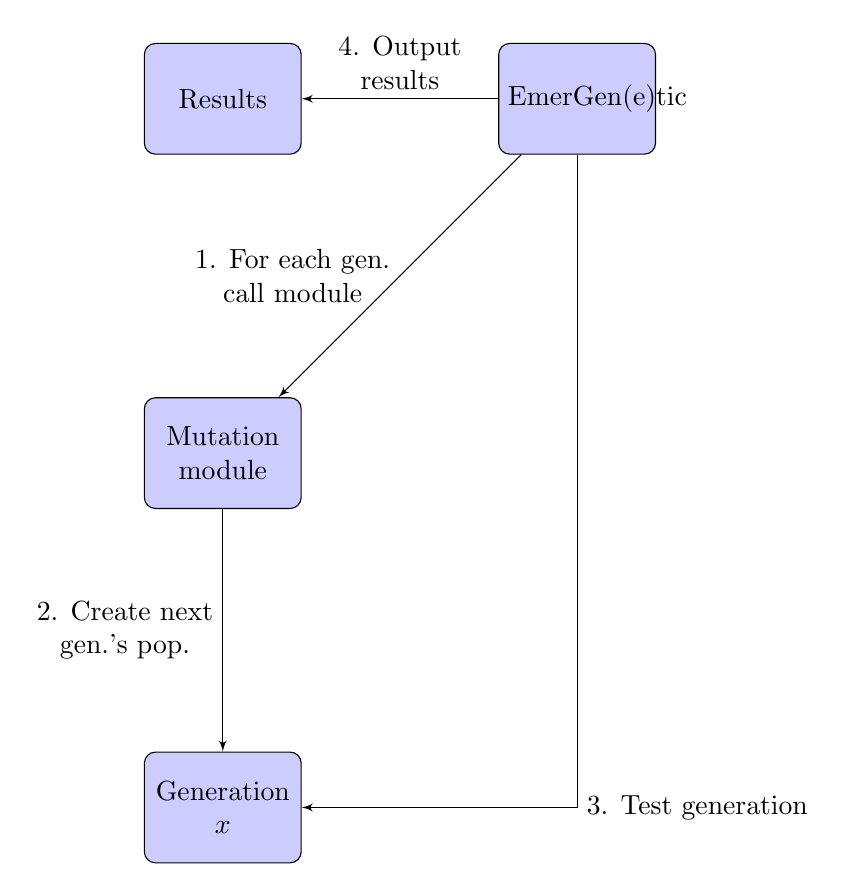
\begin{tikzpicture}[node distance = 4.5cm, auto]
			    % Place nodes
			    \node [block] (init) {EmerGen(e)tic};
			    \node [block, left of=init] (results) {Results};
			    \node [block, below of=results] (script) {Mutation module};
			    \node [block, below of=script] (generation) {Generation $x$};
			    % Draw edges
			    \path [line] (init) -- (script) node[midway,left,align=center] {1. For each gen.\\call module};
			    \path [line] (script) -- (generation) node[midway,left,align=center] {2. Create next\\gen.'s pop.};
    			 \path [line] (init) |- (generation) node[midway,right,align=center] {3. Test generation};
    			 \path [line] (init) -- (results) node[midway,above,align=center] {4. Output\\results};
			\end{tikzpicture}
			\end{center}
			
		\subsection{The Web Server}
			
			\subsubsection{How a web server works}
			
				A \textit{web server} is a type of computer. It can receive requests from other computers (called `clients') for the files that are located within it via a number of methods, usually across an Internet connection, such as HTTP. Once it has received a request, which will contain the name of the file requested, it searches its file storage for a match. If it finds it, it sends the data of the file back to the client. If it does not, it should return a message that the client knows to interpret as an error message. Below is a flowchart of how a web server works:\\
				\begin{center}
				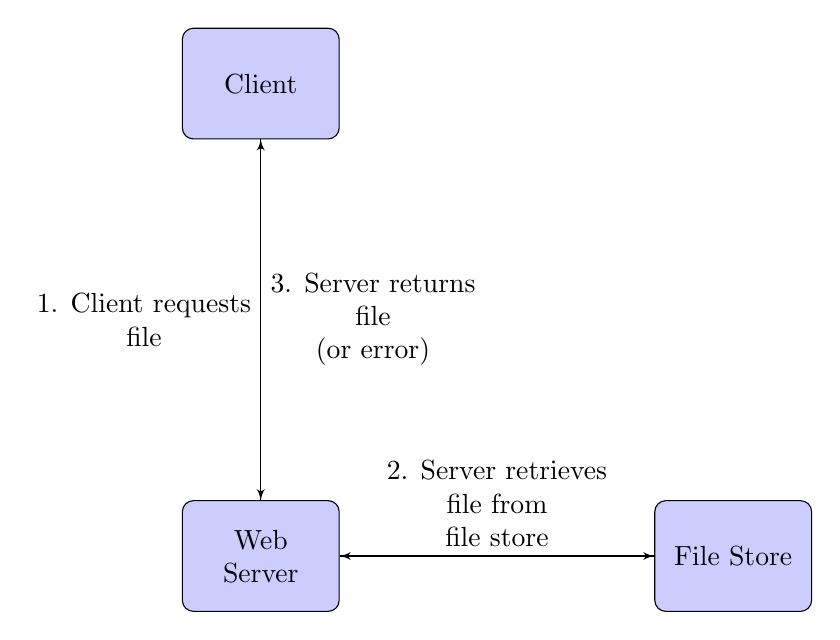
\begin{tikzpicture}[node distance = 6cm, auto]
				    % Place nodes
				    \node [block] (client) {Client};
				    \node [block, below of=client] (webserver) {Web Server};
				    \node [block, right of=webserver] (file) {File Store};
				    % Draw edges
				    \path [line] (client) -- (webserver) node[midway,left,align=center] {1. Client requests\\file};
				    \path [line] (webserver) -- (file) node[midway,above,align=center] {2. Server retrieves\\file from\\file store};
	    			 \path [line] (file) -- (webserver);
	    			 \path [line] (webserver) -- (client) node[midway,right,align=center] {3. Server returns\\file\\(or error)};
				\end{tikzpicture}
				\end{center}
			
			\subsubsection{Added extras}
		
				This is the most basic form of web server---for every request, it trawls through its files for a match and then returns that to the client. However, there are numerous extra functions that can be added to improve performance, and which can be combined to best suit various situations. For example, files can be compressed through various schemes in order to reduce their filesize before sending, and then decompressed at the client's end, which shortens the amount of time taken to transmit the (now-smaller) file.\\
				However, the one most relevant to this project is \textit{caching}. In caching, a cache is kept---this is a section of storage that is faster to retrieve data from than the regular file store, but which does not have the size to hold the full file store. When a file is returned for a client's request, it is also added to the cache. This means that if a client then requests the same file again, it will be found within the cache and returned faster than if the entire file store had to be searched.\\
				Obviously, the cache will at some point fill up. At this point, various policies for updating a full cache can be implemented. The simplest is to simply start again at the beginning and overwrite the first item. More complex ones can bring in variables like which file was requested least recently, or has been requested the fewest times, in order to try and improve speed. Again, different policies suit different situations, and there is no `magic bullet'.
				
			\subsubsection{A tale of two web servers}
			
				The present project is based off of Filho \& Porter's Dana web server code. Their project includes a client program, which is given a list of files grouped by various criteria (e.g. all large files, all image files, mixtures of both, etc.). It then sends the server program HTTP requests for each file in the list until it reaches the end. In this particular version of the software Filho \& Porter's PAL system is implemented, meaning every possible configuration found is tried---this means that each file is tested with every combination of the provided caching and compression methods, and the response time of the server (in ms) recorded. This response time is the metric by which the PAL system ranks various configurations.\\
				The goal of Filho \& Porter's project was to demonstrate improvements in file handling when using different combinations of policies for different types of request patterns. However, for the present project, the system is too complex to control all of the independent variable required for the tests to be run. As such, the scope of inquiry had to be limited to caching policy only. As such, much of Filho \textit{et al.}'s server project code was removed. This left only the caching functionality and some remnants of the web server code.
		
		\subsection{Caching}
		\label{sec:caching}
		
			Cache behaviour is located within the \lstinline|/cache/CacheHandler*.dn| family of components. Filho \& Porter's server code contains six \lstinline|CacheHandler*| variants, each with different policies for determining which item in a full cache---represented by a fixed-size array---to replace with a newly-requested file, as well as a simple cache system in which the cache is only one item long. The other methods are:
			\begin{itemize}
				\item serial replacement, where each item in turn is replaced, returning to the first item upon reaching the end of the array,
				\item most- and least-frequently used,
				\item most- and least-recently used. 
			\end{itemize}
			For example, \lstinline|CacheHandlerMFU.dn| contains the policy for replacing the most-frequently used cache item.\\
			Within each of these variant cache handling policy files there is necessarily a lot of duplicated code. Common to all variants are the method signatures (but not bodies) for:
			\begin{itemize}
				\item \lstinline|updateCache()|, which updates a full cache using the variant's specified policy,
				\item \lstinline|clearCache()|, which clears the cache completely, and
				\item \lstinline|getCachedResponse()|, which returns either the item that was received from the cache or \lstinline|null| to the caller.
			\end{itemize}
			Cache initialisation is handled as a conditional within \lstinline|updateCache()| (i.e. if there is no cache present, it creates one and places the current item in cache index 0).\\
			There are also a series of functions that are only present in individual \lstinline|CacheHandler| files, such as \lstinline|mostRecentlyUsed()| in \lstinline|CacheHandlerMRU.dn|. This does what is says on the tin, returning the most recently-used item from the cache to be overwritten. Another example is \lstinline|random()| (within \lstinline|CacheHandlerR.dn|), which unsurprisingly returns a random item from the cache.\\
			For the genetic algorithm to work it needs a base file. The base file requires all of the common functionality present and marked as out-of-bounds for the genetic algorithm. Included in these out-of-bounds methods would be the full complement of methods such as \lstinline|mostRecentlyUsed()|, which could be called upon or not as decided by a given output program.
		
		\subsection{The `Cache Policy' Genetic Algorithm}
		
			The basic workings of a genetic algorithm were covered in \S \ref{sec:introduction}, but here the specifics of the algorithm as applied to this project shall be outlined.\\
			As this project is concerned only with modifying cache updating behaviour, and thus in how to produce an index value given differing formulae, the most important line is line 110 of \lstinline|CacheHandlerBase.dn|:
			\begin{lstlisting}[language=Java]
				index = 0
			\end{lstlisting}
			The formula on the right-hand side of that assignment is the scope for mutation. From that initial `\lstinline|0|' must sprout new formulae---these formulae are what is referred to in the remainder of this report as \textit{chromosomes}. A single \textit{generation} will consist of multiple \lstinline|CacheHandler*.dn| files (or \textit{candidates}), each of which will contain a single chromosome. Within each generation, therefore, shall exist multiple distinct chromosomes. Each of these sets of chromosomes is known as the generation's \textit{population}.\\
			As mentioned before, the basic tools of a genetic algorithm are the operations of \textit{mutation} and \textit{crossover}, which shall be discussed below (along with a heuristic known as `elite selection'):\\
			
			\noindent\textbf{Mutation}\\
			
			\noindent In mutation, a section of chromosome $A$ is replaced with a new value. For example, from the example chromosome `\lstinline|0|', an operand mutation operation could change it to `\lstinline|4|'. For the mutation within the scope of this project, four types of mutation were implemented:
				\begin{itemize}
					\item binary operator mutation (e.g. `\lstinline|2+4|' into `\lstinline|2*4|'),
					\item operand mutation,
					\item unary operator mutation (e.g. `\lstinline|nthMostRecentlyUsed(2)|' into `\lstinline|nthMostFrequently- Used(2)|'), and
					\item subtree creation (e.g. `\lstinline|2+2|' into `\lstinline|2+(4*2)|').
				\end{itemize}
				The first three simply randomly change elements of the chromosomes in the hopes of finding particularly efficacious variants. The fourth, however, serves the vital role of allowing the chromosomes---which all start as `\lstinline|0|'---to increase in complexity.\\
				
			\noindent\textbf{Crossover}\\
			
			\noindent In crossover, two chromosomes $A$ and $B$ are selected. A random section of $A$ ($A'$) is then taken and inserted at a random point of $B$ ($B'$) to produce a new chromosome $C$. For example, take
				\begin{gather*}
					A = \text{ \lstinline|2+(4+3)|}\\
					B = \text{ \lstinline|4*3|}
				\end{gather*}
				and an $A'$ of `\lstinline|+(4+3)|' and a $B'$ between the `\lstinline|4|' and the `\lstinline|*|'---we produce
				\begin{gather*}
					C = \text{ \lstinline|4+(4+3)*3|}
				\end{gather*}
				Variants of crossover also exist, such as multi-point crossover (where multiple $A'$s are copied over to multiple $B'$s). However, for this project, only single-point crossover was implemented due to time constraints.\\
				
			\noindent\textbf{Elite Selection}\\
			
			\noindent There are a number of time-saving tactics (or \textit{heuristics}) that can be used to speed up the performance of a genetic algorithm. One such heuristic, implemented within this project, is \textit{elite selection}. This takes an arbitrary percentage of top-performing chromosomes for any generation (in this instance, the top 10 \%) and copies them across to the next generation unchanged. This ensures that optimal solutions are not simply discarded upon the next generation.
		
	\newpage
	
	\section{Implementation: EmerGen(e)tic}
	\label{sec:implementation}
	
		This section contains a more technically-detailed overview of the implementation of the EmerGen(e)tic program.
		
		\subsection{Folder Structure}
		
			The base folder structure for EmerGen(e)tic is as follows:
			\begin{itemize}
				\item \lstinline|/archives/|, where archives of test run data go when after completion of a script's run,
				\item \lstinline|/project/|, which contains the mutation project modules,
				\item \lstinline|/resources/|, which contains Dana overhead,
				\item \lstinline|/results/|, which contains per-generation and per-script results files and
				\item \lstinline|/scripts/|, which contains \lstinline|.script| files for running through multiple tests, grouped by some criterion/criteria.
			\end{itemize}
			
		\subsection{\lstinline|emergenetic.dn|}
		
			This Dana file contains the framework for running and testing genetic algorithm projects.\footnote{See Appendix \ref{appendix:emergen}} Passed to it are a number of command-line arguments, including the module to load and the number of generations to test.
			
			\subsubsection{\lstinline|App:main()|}
			
				The program is entered through the \lstinline|App:main()| method, whereupon the passed arguments are validated---if any are invalid, detailed error messages are output and the program terminates. The method runs the setup file \lstinline|setup.sh| from within the passes module directory (and passes the result to a variable of type \lstinline|RunStatus|, which can be helpful for debugging), and then iterates through each generation. For each generation, it runs the given module's \lstinline|mutator.py| program, followed by the \lstinline|runGeneration()| method.\\
				Upon successfully finishing the iteration of each generation, the program exits with a code of `0'---in the event of invalid arguments, it exits with a code of `1'.
	
			\subsubsection{\lstinline|runGeneration()|}
			
				The \lstinline|runGeneration()| calls the \lstinline|runCandidate()| method for each candidate within the given generation. Once this is done, it appends a newline to the \lstinline|results.csv| file within the \lstinline|results| directory.
				
			\subsubsection{\lstinline|runCandidate()|}
			
				This is the point at which a future developer will implement their own code for running and testing candidates for their own projects. In the base release of \lstinline|emergenetic.dn|, it is left blank.
				
			\subsubsection{\lstinline|printResults()|}
			
				This method prints the results of each test run to output. It then also appends the results of the run to the per-generation results file \lstinline|results|$x$\lstinline|.txt|, and to the per-script results file \lstinline|results.csv| within the \lstinline|results| directory.
	
	\newpage
	
	\section{Implementation: \lstinline|cachingpolicy|}
	\label{sec:cachingpolicyimpl}
		
		In this section, the technical implementation of the \lstinline|cachingpolicy| module used for this project is detailed.
		
		\subsection{Folder Structure}
			
			In addition to the base folder structure of EmerGen(e)tic, the following directories were added.
			\begin{itemize}
				\item \lstinline|/cache/|, where the generations of various \lstinline|CacheHandler*.dn| files are kept, each within a directory numbered with their generation number and in files of the format \lstinline|CacheHandler|$x$\lstinline|_|$y$\lstinline|.dn|, where $x$ is the number of the generation and $y$ is the number of the candidate,
				\item \lstinline|/cachebackup/|, which contains a fresh copy of \lstinline|CacheHandlerBase.dn| for quickly clearing the \lstinline|/cache/| directory after a full test run,
				\item \lstinline|/htdocs/|, which contains all the files to request from the web server,
				\item \lstinline|/project/cachingpolicy|, which contains the files for the \lstinline|cachingpolicy| module and
				\item \lstinline|/resources/cache|, which contains the Dana specifications for the caching components.
			\end{itemize}
			
		\subsection{Genetic Algorithm search space}
		
			Before a genetic algorithm can be implemented, the search space must be defined:
			\begin{gather*}
				 \text{Let }c\text{ represent the cache length} \\
				 \text{Let }l\text{ represent an AST leaf values} \\
				 \text{Let }n\text{ represent an AST node values} \\\\
				 l \in \mathbb{N} \\
				 n \in \left\{\times, +, -, \div, MostFrequent\left(\right), MostRecent\left(\right), Rand\left(\right) \right\} \\\\
				 \text{Let }a\left(n\right)\text{ be a function that returns the arity of function }n \\
				 \text{Let }r\text{ represent the result of }n\left(\right)\text{, }n\left(l\right)\text{ or }n\left(l_1, \dots, l_{a\left(n\right)}\right) \\
				 \text{Let }i\text{ represent the cache index value to replace} \\\\
				 r\in \mathbb{N} \\
				 i \in \left\{x \in \mathbb{N} : 0 \leq i \leq c-1\right\} \\
				 \therefore i = r \bmod{\left(c-1\right)}
			\end{gather*}\\
			In real terms then, the the set of actual Dana operators and methods $n_{Dana}$ used was
			\[ n_{Dana} \in \left\{\text{\lstinline|*|}, \text{\lstinline|+|}, \text{\lstinline|-|}, \text{\lstinline|/|}, \text{\lstinline|nthMostFrequentlyUsed()|}, \text{\lstinline|nthMostRecentlyUsed()|}, \text{\lstinline|random()|}\right\} \]
			and the resolve flag $res$, which was passed through to \lstinline|nthMostFrequentlyUsed()| and \lstinline|nthMostRecentlyUsed()| as a constant in each individual program, was of the value
			\[res \in \left\{\text{\lstinline|n|}, \text{\lstinline|o|}, \text{\lstinline|r|}\right\}\]
			
		\subsection{\lstinline|CacheHandlerBase.dn|}
			
			From the various \lstinline|CacheHandler*.dn| files within Filho \& Porter's \lstinline|/cache/| were distilled the common elements of each (the methods covered in \S \ref{sec:caching}), collected into one file.\footnote{See Appendix \ref{appendix:base}} 

			\subsubsection{\lstinline|CacheHandler:getGetCachedResponse()|}
			
				This method returns an item specified in a request from the cache if it exists there---otherwise, it returns \lstinline|null|.

			\subsubsection{\lstinline|CacheHandler:updateCache()|}
				
				This method updates the cache if a requested item is not already in it. If the cache is full, this method contains the formula for determining the cache index to replace. Lines 70--71---demarcated with the comments \lstinline[language=Java]|// BEGIN| and \lstinline[language=Java]|// END|---indicate to the genetic algorithm its bounds of operation. Within these lines, the method for determining cache index $i$ is determined for each chromosome.
			
			\subsubsection{\lstinline|CacheHandler:clearCache()|}
			
				This method clears the cache completely.
			
			\subsubsection{\lstinline|nthMostFrequentlyUsed()|, \lstinline|nthMostRecentlyUsed()| \& \lstinline|random()|}
			
				These methods return the item in the cache that fits their criterion (or, in the case of \lstinline|random()|, a random item). Including all of the various most/least frequently/recently used methods would lead to an unnecessarily large file, so they were generalised into the methods \lstinline|nthMostFrequentlyUsed()| and \lstinline|nthMostRecentlyUsed()|, which each take their $n$ as an argument.
				
			\subsubsection{\lstinline|resolve()|}
			
				The \lstinline|resolve()| method takes a flag indicating how to resolve the situation of multiple returns from one of the aforementioned three methods (e.g. in the event that the least-frequently used file is not the only file in the cache with that number of hits). The flag can be set to return either the newest item, the oldest or a random choice.
			
		\subsection{\lstinline|emergenetic.dn|}
		
			Within the \lstinline|runCandidate()| method,\footnote{See Appendix \ref{appendix:runcand}} the \lstinline|CacheHandler| component within \lstinline|CacheHandler*.dn| is loaded using Dana's \lstinline|RecursiveLoader|, which ensures that all of its dependencies are also loaded. A timer is started and each file within the given script file is requested from the web server. When the script file is finished, the timer is stopped and the overall time taken (and that the value represented ms) is passed to \lstinline|printResults()|. As \lstinline|RecursiveLoader| lacks an \lstinline|unload()| method, each of the loaded components is then looped through and \lstinline|unload()| called on them in turn.
		
		\subsection{\lstinline|cachingpolicy/mutator.py|}
		\label{sec:python}
		
			This Python file contains the genetic algorithm logic for the \lstinline|cachingpolicy| module.\footnote{See Appendix \ref{appendix:genetic}} It can be run as a standalone Python script or imported as a Python module into other projects.
		
			\subsubsection{\lstinline|getSubLists()|}
			
				This method recursively produces a \lstinline|List| of nested \lstinline|List|s representing every subtree present within a given chromosome (i.e. every bracketed expression).
			
			\subsubsection{\lstinline|crossover()|}
			
				This method performs single-point crossover between two chromosomes passed to it as arguments $A$ and $B$. It first calls \lstinline|getSubLists()| on $A$ in order to get a \lstinline|List| of all the possible subtrees of $A$. It then randomly chooses points within $B$ until it finds an operand token, at which point it replaces the operand with a randomly-chosen \lstinline|List| from $A$.
			
			\subsubsection{\lstinline|mutate()|}
			
				This method performs four distinct multiple-point mutations. If it is the first run it imports the individual mutation probabilities from \lstinline|config.conf|, and if it is the initial population it overrides the mutation probability to be 100 \%. It then recursively iterates over each token in the chromosome and has a chance to possibly apply one of the mutation operations. The recursive element comes in when it encounters a token of type \lstinline|List| (i.e. a bracketed expression), in which case it calls \lstinline|mutate()| upon the sublist.
			
			\subsubsection{\lstinline|parse()| \& \lstinline|compile()|}
			
				The former of these methods takes an expression as a string (e.g. `\lstinline|2+(4*2)|') and returns a \lstinline|List| representation (with nested \lstinline|List|s for bracketed expressions). The latter takes such a \lstinline|List| and returns the original string expression.
				
			\subsubsection{\lstinline|createInitialPop()|}
			
				If the python script is called with a generation argument of `0' it calls the \lstinline[language=python]|createInitialPop()| method first. This creates an initial population by copying over \lstinline|CacheHanderBase.dn| and applying \lstinline[language=python]|mutate()| to each candidate with a 100 \% mutation probability.
			
			\subsubsection{\lstinline|readChromosomeFromFile()| \& \lstinline|writeChromosomeToFile()|}
			
				These methods are simple utility methods for reading and writing chromosomes from and to \lstinline|CacheHandler*.dn| files.
			
			\subsubsection{\lstinline|hasSubTrees()|}
			
				This method returns a boolean indicating whether a passed chromosome has nested expressions or not.
			
			\subsubsection{\lstinline|main()|}
			
				The \lstinline|main()| method takes the $n$ candidates of previous generation $m$ (passed to it as arguments) and selects the top 10 \% of them to go across unchanged to generation $m+1$. Of the remainder, probabilities of mutation and crossover are applied to each and, when those occur, separate probabilities determine the type of mutation or crossover that will occur.
				
		\subsection{\lstinline|cachingpolicy/config.conf|}
			
			\lstinline|mutator.py| reads in its probability values from the file \lstinline|config.conf|.\footnote{For an example \lstinline|config.conf|, see Appendix \ref{appendix:settings}} This file contains a number of name-value pairs. The left hand side of each config. pair is ignored by \lstinline|mutator.py| and is thus present only for the aid of the human user.

	\newpage
	
	\section{The System in Operation}
	
		In this section is outlined the process of creating a new module---and running a suit of tests using it---via the EmerGen(e)tic framework.
			
		\subsection{Creating a Module}
			
			\subsubsection{Files}
			
				To create a new module for a future research project, create the folder within the \lstinline|project| directory. Within this directory, create a Python file \lstinline|mutator.py|, which will contain all of your genetic algorithm and a Bashscript file \lstinline|setup.sh| to perform any functions prior to each test such as creating or deleting folders (this may not perform any tasks, but the file must still be present).\footnote{For an example \lstinline|setup.sh|, see Appendix \ref{appendix:setup}}

			\subsubsection{Implementation}
			
				To implement the new module and test the results of it, code must be written within the \lstinline|runCandidate()| method of the Dana file \lstinline|emergenetic.dn|. Within this method will be defined the process of testing, how to use script files and the metric by which success is measured. The other methods within the file will remain unchanged.
					
		\subsection{Creating Scripts}
		
			In order to run a suite of different tests for each candidate, scripts are required. In the \lstinline|cachingpolicy| instance, these script files contain the filenames of different files grouped by some property or properties. For example, \lstinline|difffile-html.script| tests a number of different files, all of which are HTML but are a mixture of sizes, whilst \lstinline|difffile.script| tests different files that are a mixture of HTML and image and have a range of sizes. This can be used to easily showcase the system producing different results that provide optimum behaviour based on different operational conditions.
						
		\subsection{Running EmerGen(e)tic}
		
			After compiling the \lstinline|emergenetic.dn| file, the program can be run. It expects four command-line arguments, and can take a fifth optional one. The command is as follows:
			\begin{lstlisting}[language=bash]
				dana emergenetic <module> <script> <generations> <candidates> [verbose]
			\end{lstlisting}
			\lstinline|<module>| is the name of the module folder that you wish to use for your tests.\\
			\lstinline|<script>| is the name of the script file for this particular test, located within the \lstinline|/scripts/| directory and without the trailing \lstinline|.script| file extension. For example, ``\lstinline|difffile|" for the script file \lstinline|difffile.script|.\\
			The \lstinline|<generations>| and \lstinline|<candidates>| arguments are the number of generations to run the test for, and the number of candidates to produce per generation.\\
			The optional \lstinline|verbose| argument, if present, produces far more verbose output text. This can be useful for debugging.\\
			For example, below is the console output for a typical run of the \lstinline|cachingpolicy| module (with the \lstinline|verbose| flag omitted):
			\begin{lstlisting}
				ben@metacom-1:~/emergenetic$ dana emergenetic cachingpolicy difffile 10 10
	
				Response time for configuration 0x0: 19 ms
				Response time for configuration 0x1: 20 ms
				Response time for configuration 0x2: 20 ms
				Response time for configuration 0x3: 19 ms
				Response time for configuration 0x4: 20 ms
				Response time for configuration 0x5: 19 ms
				Response time for configuration 0x6: 20 ms
				Response time for configuration 0x7: 19 ms
				Response time for configuration 0x8: 19 ms
				Response time for configuration 0x9: 20 ms
				
				Response time for configuration 1x0: 20 ms
				Response time for configuration 1x1: 20 ms
				Response time for configuration 1x2: 19 ms
				Response time for configuration 1x3: 19 ms
				Response time for configuration 1x4: 19 ms
				Response time for configuration 1x5: 19 ms
				Response time for configuration 1x6: 20 ms
				Response time for configuration 1x7: 20 ms
				Response time for configuration 1x8: 19 ms
				Response time for configuration 1x9: 19 ms
				
				Response time for configuration 2x0: 20 ms
				Response time for configuration 2x1: 19 ms
				Response time for configuration 2x2: 20 ms
				Response time for configuration 2x3: 20 ms
			\end{lstlisting}
			...and so on. Here is a sample of console output with the \lstinline|verbose| flag included:
			\begin{lstlisting}
				ben@metacom-1:~/emergenetic$ dana emergenetic cachingpolicy difffile 10 10 verbose
				
				Response time for configuration 0x0: 20 ms
				Response time for configuration 0x1: 19 ms
				Response time for configuration 0x2: 19 ms
				Response time for configuration 0x3: 19 ms
				Response time for configuration 0x4: 19 ms
				Response time for configuration 0x5: 20 ms
				Response time for configuration 0x6: 20 ms
				Response time for configuration 0x7: 19 ms
				Response time for configuration 0x8: 20 ms
				Response time for configuration 0x9: 20 ms
				
				Applying rank selection to top 10% from prev. generation...
				        Result: 0_2 copied to 1_2
				
				Mutating 0_3->1_3:
				        Mutating: 0
				                Result: 0*0
				        Mutating: 0*0
				                Result: 0/0
				        Mutating: 0/0
				                Result: 0/random()
				0_3->1_3 mutation finish.
				
				Mutating 0_4->1_4:
				        Mutating: 0
				                Result: 0*1
				        Mutating: 0*1
				                Result: 0*1
				        Mutating: 0*1
				                Result: 0*nthMostFrequentlyUsed(0)
				0_4->1_4 mutation finish.
				
				Mutating 0_5->1_5:
				        Mutating: 0
				                Result: 0-1
				        Mutating: 0-1
				                Result: 0-1
				        Mutating: 0-1
				                Result: 0-17
				0_5->1_5 mutation finish.
			
				Response time for configuration 1x0: 19 ms
				Response time for configuration 1x1: 29 ms
			\end{lstlisting}
			...and so on.
			
		\subsection{Background Tests}
		
			The process can be run as a background process so that the Terminal window/SSH connection can be closed by the user without interrupting the tests. The user can either run the EmerGen(e)tic program itself as a background process, or write a script to run.\footnote{An example script can be seen in Appendix \ref{appendix:bash}} To run the process in the background, use the commands
			\begin{lstlisting}[language=bash]
				dana emergenetic cachingpolicy difffile 10 10 &>/dev/null &
				disown
			\end{lstlisting}
			By redirecting output to \lstinline|output.txt| rather than \lstinline|/dev/null|, the user can also track the progress of the tests as they happen.
	
	\newpage
		
	\section{Testing \& Evaluation}
	\label{sec:testing}
	
		In this section is outlined the results of various testing of the system. Following that, the successes and failures of the project will be reviewed and how well it satisfies the research goals outlined in \S \ref{sec:introduction} assessed.
		
		\subsection{Testing EmerGen(e)tic}
		
			The first test was one to make sure that the EmerGen(e)tic program was working as expected. Using a very simple \lstinline|helloworld| module (that simply took a \lstinline|.txt| file containing the line `Hello world' and applied a random chance of mutating the letters into others), three tests were run.\footnote{See Appendix \ref{appendix:helloworld}}\\
			The first test, with mutation probability set to 50 \%, produced the following output:
			\lstinputlisting[lastline=15]{../dat/helloworld/output50.txt}
			\begin{lstlisting}
			[...]
			\end{lstlisting}
			\lstinputlisting[firstline=60,lastline=65]{../dat/helloworld/output50.txt}
			As you can see, mutations were successfully applied to some (but not all) candidates on each generation's run, with the generations further from 0 being progressively less recognisable from their origins.\\
			In order to test that the system worked too with varying probability values, tests were run with probability values of 0 \% and 100 \%.\\
			For 0 \%, the results were as follows:
			\lstinputlisting[lastline=20]{../dat/helloworld/output0.txt}
			\begin{lstlisting}
			[...]
			\end{lstlisting}
			\lstinputlisting[firstline=60,lastline=65]{../dat/helloworld/output0.txt}
			This shows that no mutation operations were applied.\\
			For 100 \%, the results were as follows:
			\lstinputlisting[lastline=20]{../dat/helloworld/output100.txt}
			\begin{lstlisting}
			[...]
			\end{lstlisting}
			\lstinputlisting[firstline=60,lastline=65]{../dat/helloworld/output100.txt}
			This shows that the mutations were applied to every single letter of every single candidate.\\
			From these, EmerGen(e)tic is shown to be able successfully implement genetic algorithms and tests thereof. Also, the speed at which modules can be developed is demonstrated: \lstinline|helloworld| took around 15 mins to write.\\
		
		\subsection{Testing \lstinline|cachingpolicy|}
		\label{sec:testingcache}
		
			\begin{wrapfigure}{l}{0.46\textwidth}
				\vspace{-20pt}
			  	\begin{center}
			    	\includegraphics[width=0.44\textwidth]{difffile-large}
					\vspace{-20pt}
			  		\caption{}
					\label{fig:difffile-large}
			    	\includegraphics[width=0.44\textwidth]{difffile-large-wo}
					\vspace{-20pt}
			  		\caption{}
					\label{fig:difffile-large-wo}
			    	\includegraphics[width=0.44\textwidth]{samefile-images}
					\vspace{-20pt}
			  		\caption{}
					\label{fig:samefile-images}
			    	\includegraphics[width=0.44\textwidth]{samefile-images-wo}
					\vspace{-20pt}
			  		\caption{}
					\label{fig:samefile-images-wo}
			  	\end{center}
				\vspace{-10pt}
			\end{wrapfigure}
			With EmerGen(e)tic itself having been demonstrated to work, answering the research questions posed in the introduction to this project could be attempted. The first question was phrased `can genetic algorithms be productively used to produce optimum components for an emergent system?'\\
			To test this hypothesis, the initial probability variables in \lstinline|config.conf| were set to the values shown in Appendix \ref{appendix:settings}---the probability of a complexity-increasing mutation was set so high in the hope that this would produce more rapidly a diverse spread of different chromosomes.\\
			Tests were then run on the test suite \lstinline|difffile-large|, which requests a series of different HTML and image files, all large. Each test was run for 18 generations, consisting of a population of 35 candidates each, and repeated three times. The results were the averaged across each of the three runs. The average result per generation is visible in Figs \ref{fig:difffile-large} \& \ref{fig:difffile-large-wo}.\\
			There were a number of anomalous results that initially made discerning a pattern difficult (e.g. candidate 14\_4 from the first run returned 410 ms). Removing any results $\geq$35 ms (only 14 out of a total of 1890 results) produced Fig. \ref{fig:difffile-large-wo}, where the trending towards faster and faster response times is more obvious. From a wider range of results for the initial few generations (21--30 ms), the components in later generations tended towards consistent level of around 21 ms response time.\\
			It wouldn't have been surprising to see that these higher-performing chromosomes shared similar characteristics, such as all calling \lstinline|nthMostFrequentlyUsed()|. Indeed, this appears to have been somewhat the case, although not exclusively so---the chromosomes `\lstinline|11/random()|' and `\lstinline|nthMostRecentlyUsed(0)*nthMostFrequentlyUsed(0)|' each achieve 21 ms, as did a range of other chromosomes. However, the most common characteristic of all of the generation 18 chromosomes seemed to be the presence of one or both of the \lstinline|nthMost*Used()| functions---29 out of the 38 chromosomes featured one of these functions, and 8 featured both.\footnote{To view all of the gen. 18 chromosomes, see Appendix \ref{appendix:chromosomes}}\\
			The test suite \lstinline|samefile-images|---which requests the same image file repeatedly---was then run with the same conditions. The results are visible in figs \ref{fig:samefile-images} and \ref{fig:samefile-images-wo}.\\
			There is no visible improvement in either of these charts. Barring two anomalous results, the response times only varied between 18 and 19 ms, suggesting that no amount of mutation made a difference on performance. This was expected, however---after enough runs, every index in the cache will point to identical data and the formula for updating the cache will be meaningless.
	
		\subsection{Evaluation}
		\label{sec:eval}
			
			The research aim specified for EmerGen(e)tic was `to produce a framework for enabling rapid development of genetic improvement tests'. This has been done---EmerGen(e)tic is simple to extend with new modules, being written in the more widely-known Python language (rather than the admittedly more niche Dana). Given a blank copy of EmerGen(e)tic and this report, it is confidently assumed that a researcher could begin deploying their own tests in minimal time. To support this claim, the \lstinline|helloworld| and \lstinline|cachingpolicy| modules were developed to demonstrate the framework in action.\\
			The \lstinline|cachepolicy| module (initially) produced results that appear to support the assertion made in \S \ref{sec:introduction}---i.e. that genetic algorithms can be usefully applied to the creation of emergent system components. As was expected too, this is not the case for all contexts (e.g. \lstinline|samefile-images|), which demonstrates that in some instances, the added overhead of running genetic algorithm generations is not rewarded with any tangible improvements.\\
			However, perhaps a scope that would have produced more variance than just cache updating behaviour would have been advisable to choose at the start of the project in order to better prove or disprove this hypothesis. As it stands, a proof, albeit a slightly weak proof, is nonetheless provided.\\
			An additional aim was set, to `repeat the tests multiple times with a variety of conditions and see what, if any, trends emerge.' However, between the tests featured in \S\ref{sec:testingcache} and when the condition-variance tests were due to be run, access to the research computer was temporarily suspended. Upon returning to it a week later, test runs (even those with identical conditions to the ones previously performed) no longer produced meaningful results---response times barely varied for all tests run, regardless of number of generations.\\
			To make sure that this was not a result of the machine's processing speed increasing and minor changes in response time being undetectable, all of the test suites were tripled in length in the hope that minor changes would become more pronounced. Unfortunately this had no effect, and at this late stage in the project no alternative was left but to cease testing of the \lstinline|cachepolicy| module.\\
			However, the approaches that would have been taken will be outlines in the `Future Improvements' section at the end of this report.
			
	\newpage
	
	\section{Conclusion}

		In \S \ref{sec:introduction}, two research questions were established. In this section, the answers provided will be considered. Then, suggestions for further research will be outlined.\\
		
		\noindent\textbf{Can genetic algorithms can be productively used to produce optimum components for an emergent system?}\\
		
		\noindent This has been shown to be the case. The response times for delivery of certain types of files have been demonstrated steadily decreasing per generation following application of genetic algorithms. However, it has also been shown that there are some instances where genetic algorithms are of little use (e.g. when the same file is requested from the web server repeatedly). In these cases, the overhead of running the genetic algorithm (and each generation takes a non-trivial amount of time to produce, compile and test) is not rewarded.\\
		
		\noindent\textbf{What are the optimal conditions for doing so (i.e. mutation probabilities, generation sizes, etc.)?}\\
			
		\noindent As explained in \S\ref{sec:eval}, issues that emerged late in the project prohibited exploration of this area.
		
		\subsection{Future Development}
		
			\subsubsection{Completing the original goal of finding the optimal conditions for the genetic algorithm}
			
				As previously mentioned, issues prevented this avenue of research from being explored. If these issues were resolved, it would be useful to revisit this second research question. The intended plan was to set the probabilities of the four specific mutation operations to 50 \%, run a test suite with mutation and crossover probabilities set at each 10-step interval (i.e. 0 \%, 10 \%, $\dots$ , 100 \%) and compare results to determine the optimum probabilities of both. This could then be re-run with the probabilities set at opposing ends (i.e. 0\% and 100 \%) and converging towards and then past each other---this would hypothetically display whether similar or distinct probabilities for the two operations (if either) are more desirable.\\
				After these tests have hopefully shown a broad region of optimal probabilities, more fine-grained testing within that region could then take place. This could involve testing the original two probabilities with a range of values across a smaller step size, or testing different combinations of probabilities for the four specific mutation operations. For example, all but one could be set to 0 \% and this used to determine how well they work in isolation.
		
			\subsubsection{Designing more modules}
			
				For a future project or projects, one could develop and run different tests using the EmerGen(e)tic framework provided here. For example, a module that applied genetic algorithms to the file compression options including in Filho \& Porter's original web server. Alternatively, such a module could be combined with another (such as \lstinline|cachingpolicy|) in order to test a broader scope of mutation than just individual functionality and demonstrate the potential interlinked effects of this.
				
			\subsubsection{A more `Danatically'-designed EmerGen(e)tic}
			
				When running an EmerGen(e)tic module in which the genetic algorithm is improperly implemented, and thus can produce uncompilable components, the compilation attempt will fail for that component and the entire EmerGen(e)tic test run/suite fail upon trying to load the non-existent component object file that has thus not been produced. Dana lacks exception-handling functionality, as a component's failure is intended to be signalled to the calling component via a \lstinline|return|. By re-designing the system in a more idiomatically Dana way and calling the tests as a separate component rather than in the \lstinline|runCandidate()| method of \lstinline|emergenetic.dn|, failure of an individual test could be ignored and the test runs continued.\\
				Another benefit of this would be the complete separation of the functionality currently within \lstinline|runCandidate()|, which module developers must edit in order to implement their modules, and the remainder of the \lstinline|emergenetic.dn| file, which they should no have cause to touch. As it stands, the \lstinline|cachingpolicy| module contains a copy of \lstinline|emergenetic.dn| with the \lstinline|runCandidates()| implementation within it, which overwrites the existing \lstinline|emergenetic.dn| within the base distribution. This raises issues---if a module is written for a specific version of \lstinline|emergenetic.dn|, upgrading it would result in extra, unnecessary workload for the developer. However, if the \lstinline|runCandidate()| functionality could thus be moved into a separate \lstinline|runCandidate.dn| file, then issues with EmerGen(e)tic versions would be resolved. Also, this would allow EmerGen(e)tic to be distributed as a black box API, without having to distribute source files (although, as the software is released under the GNU GPLv3, this last point is less relevant), as well as allowing a user to install multiple modules simultaneously.
				
			\subsubsection{Issues within the present \lstinline|cachingpolicy| module}
			
				Besides the issues that prohibited testing for optimum conditions, there were a couple other outstanding issues within the \lstinline|cachingpolicy| modules that could be fixed in the future.\\
				Foremost of these is that test runs will sometimes, with what appears to be no predictability, stop outputting just after finishing a generation but continue to run, draining system resources until the process is killed. \lstinline|python| can be seen to still be running which, along with the stage in the process where the issue occurs and the lack of an output error message, suggests that the fault may lie in the \lstinline|cachingpolicy| module. The nature of the issue would further suggest an endless loop occurring somewhere---thus, suspicions fall upon the \lstinline|while| loop within the \lstinline|crossover()| method, or the recursive elements of the \lstinline|crossover()| and \lstinline|mutation()| methods.
				
			\subsubsection{Putting human developers further out of work (through meta-learning)}
			
				Finally, and potentially the most interesting avenue for further research of the system based on the problem it set out to fix (as outlined in \S \ref{sec:introduction}): meta-learning.\cite{meta} In this case, the system would have an ability not just to rank candidates by a predefined metric (in \lstinline|cachingpolicy|'s case the response time in ms), but also to change its metric using the same principles of genetic improvement. Despite removing the human developer from much of the software development via the implementation of genetic algorithms, one is still required to write those algorithms and, most egregiously, outline the metric(s) by which performance is measured. If the system could be left to improve its own algorithm and, if a candidate was found, amend how it judges success of candidates, the goal of the programmerless system will have been even further achieved.
		
	\newpage
	
	\bibliographystyle{IEEEtran}
	\bibliography{final-report}	
	
	\newpage
	
	\appendices
	
		\section{\lstinline|emergenetic.dn|}
		\label{appendix:emergen}
		\lstinputlisting[language=Java]{../src/emergenetic/emergenetic.dn}
	
		\newpage
		
		\section{\lstinline|helloworld/mutator.py|}
		\label{appendix:helloworld}
		\lstinputlisting[language=Python]{../src/helloworld/project/helloworld/mutator.py}
			
		\newpage
		
		\section{\lstinline|cachingpolicy|}
			\subsection{\lstinline|CacheHandlerBase.dn|}
			\label{appendix:base}
			\lstinputlisting[language=Java]{../src/cachingpolicy/cachebackup/CacheHandlerBase.dn}
			
			\newpage
			
			\subsection{\lstinline|mutator.py|}
			\label{appendix:genetic}
			\lstinputlisting[language=Python]{../src/cachingpolicy/project/cachingpolicy/mutator.py}
			
			\subsection{\lstinline|emergenetic.dn|'s \lstinline|runCandidates()| method}
			\label{appendix:runcand}
			\lstinputlisting[language=Java, firstline=131, lastline=173]{../src/cachingpolicy/emergenetic.dn}
			
			\subsection{\lstinline|setup.sh|}
			\label{appendix:setup}
			\lstinputlisting[language=bash]{../src/cachingpolicy/project/cachingpolicy/setup.sh}
			
			\subsection{\lstinline|config.conf|}
			\label{appendix:settings}
			\lstinputlisting{../src/cachingpolicy/project/cachingpolicy/config.conf}
			
			\subsection{Gen. 18 chromosomes}
			\label{appendix:chromosomes}
			\lstinputlisting[language=Java]{../dat/cache/difffile-large/17/chromosomes.txt}
		
		\newpage
		
		\section{\lstinline|runTests.sh|}
		\label{appendix:bash}
		\lstinputlisting[language=bash]{../dat/runTests.sh}

\end{document}